\documentclass[reprint,amsmath,amssymb,aps,prl,superscriptaddress,floatfix]{revtex4-2}

\usepackage{bm}
\usepackage{graphicx}
\usepackage{microtype}
\usepackage{xcolor}
\usepackage[colorlinks=true,linkcolor=blue!50!black,citecolor=blue!50!black,urlcolor=blue!50!black]{hyperref}

\graphicspath{{figures/}}

\newcommand{\Jzz}{J_{zz}}
\newcommand{\Jpm}{J_{\pm}}
\newcommand{\ghex}{g_{\mathrm{hex}}}
\newcommand{\gfour}{g_4}
\newcommand{\bq}{\bm q}
\newcommand{\br}{\bm r}
\newcommand{\bdelta}{\bm\delta}
\newcommand{\ice}{\mathcal I}

\begin{document}

\title{Winding-Free Exact Diagonalization of Quantum Spin Ice}

\author{Z.-B.~Zhou}
\affiliation{Department of Physics, [institution], [city], [country]}

\date{\today}

\begin{abstract}
Extracting quantum-spin-ice dynamics from thermodynamics requires finite
clusters precisely where periodic boundaries generate a nonbulk process.
On the 32-site pyrochlore torus, a four-spin loop returns to the ice manifold
at order $J_\pm^2/J_{zz}$, parametrically before the physical six-spin ring at
order $|J_\pm|^3/J_{zz}^2$.  We assign every virtual sequence a
gauge-invariant transported dipole and project its zero translation
character before diagonalization.  Through third order, this removes all 24
wrapping four-loops and 96 wrapping hexagons while preserving all 32
contractible hexagons and their amplitudes.  An equivalent polarization
mask makes the construction directly executable on the 2,970-state FCC-32
ice manifold.  Operator counts, spectral collapse, heat capacity, and
dynamical correlations establish that the projection removes the lower-order
channel without suppressing physical ring dynamics.  For Ce$_2$Hf$_2$O$_7$,
the published linked-cluster parameters place the clean ring peak at
$7.1$ mK rather than the observed $25$ mK.  Enforcing both scales yields a
new high-temperature-moment-preserving parameter target for a joint refit.
\end{abstract}

\maketitle

The two heat-capacity maxima of Ce$_2$Hf$_2$O$_7$, near $65$ and $25$ mK,
sharpen a general numerical problem in quantum spin ice (QSI)
\cite{Smith2025}.  Numerical linked-cluster expansion (NLC) constrains the
exchange parameters from the higher-temperature line shape, whereas the
lower feature lies at the scale where tunneling within the ice manifold
should become coherent.  In QSI, the ice rule is an emergent Gauss law and
hexagonal ring exchange generates the low-energy $U(1)$ gauge dynamics
\cite{Hermele2004,Gingras2014,Benton2012}.  Relating the two temperature
scales therefore requires a controlled low-energy calculation.  This is
particularly important for the
dipolar--octupolar pyrochlores, where candidate $U(1)_\pi$ regimes are not
accessible to sign-free quantum Monte Carlo and exact diagonalization (ED)
remains one of the few unbiased dynamical tools
\cite{Gaudet2019,Gao2019,Sibille2020,Smith2022,Poree2025}.

The standard 32-site periodic cluster is not innocuous in this regime.  Its
torus contains short alternating paths that do not exist in the infinite
pyrochlore lattice.  Most seriously, a four-spin path closes through a
periodic identification and mixes ice configurations one perturbative order
before the physical hexagonal ring.  The error consequently grows relative
to the desired signal as the ice expansion becomes more accurate.  Neither
increasing spectral resolution nor averaging observables over boundary
twists identifies the offending virtual process.  What is needed is an
operator-level criterion that distinguishes bulk-contractible from
boundary-wrapping transport.

Here we derive such a criterion and turn it into a finite-cluster protocol.
Every virtual exchange sequence carries a translation character measured by
its transported spin dipole.  Its zero-character component is precisely the
part that can be embedded without winding.  We first expose the finite-size
failure, then prove that this projection deletes the spurious four-site
channel while retaining the physical six-site ring with unchanged
coefficient.  Independent matrix-element, thermodynamic, and spectroscopic
tests establish that the operation cleans the topology rather than the
physics.  We finally combine the resulting low-energy scale with the NLC
constraint on Ce$_2$Hf$_2$O$_7$.

We use gauge-adapted axes and begin with
\begin{equation}
 H=\Jzz\sum_{\langle ij\rangle}S_i^zS_j^z
 -\Jpm\sum_{\langle ij\rangle}(S_i^+S_j^-+S_i^-S_j^+),
 \qquad \Jzz>0 .
\label{eq:model}
\end{equation}
Up to a constant, the Ising term is
$H_0=(\Jzz/2)\sum_tQ_t^2$, where $Q_t=\sum_{i\in t}S_i^z$.  The ice manifold
$\ice$ has $Q_t=0$.  A single term in $V$ creates two charged tetrahedra, so
$PVP=0$.  On the infinite lattice the shortest alternating cycle is a
hexagon.  Three exchanges annihilate the intermediate charges and produce
the leading off-diagonal matrix element
\begin{equation}
 \ghex=12|\Jpm|^3/\Jzz^2.
\label{eq:ghex}
\end{equation}
The $2\times2\times2$ primitive FCC torus instead contains 24 four-site
cycles, all noncontractible.  Two exchanges along either perfect matching
return to $\ice$ with amplitude
\begin{equation}
 \gfour=4\Jpm^2/\Jzz,\qquad
 \frac{\gfour}{\ghex}=\frac{\Jzz}{3|\Jpm|}.
\label{eq:g4}
\end{equation}
Thus the torus artifact is not a small correction to the bulk ring: it is
parametrically larger by $\Jzz/(3|\Jpm|)$ in the controlled Ising limit.

\begin{figure*}[t]
\centering
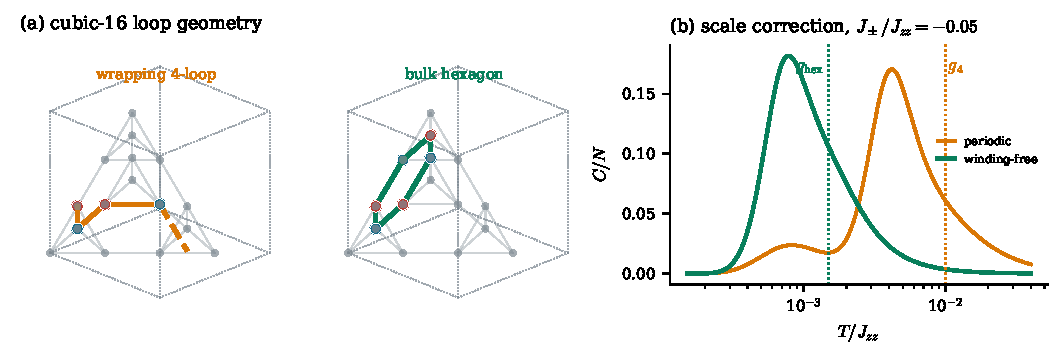
\includegraphics[width=\textwidth]{fig1_fcc32_origin.pdf}
\caption{\textbf{Origin and thermodynamic consequence.}
(a) Orthographic views of the conventional $1\times1\times1$ cubic-16 cell.
The four-site exchange closes through the boundary (dashed segment), whereas
the six-site hexagon is contractible. (b) On FCC-32 at
$\Jpm/\Jzz=-0.05$, the periodic heat-capacity maximum follows the
second-order scale $\gfour$; zero-transport projection moves it to the
third-order gauge scale $\ghex$.}
\label{fig:origin}
\end{figure*}

Figure~\ref{fig:origin}(a) uses the cubic-16 cell only to show the two paths
in an uncluttered orthographic geometry.  Every many-body result below uses
FCC-32: 32 spins, 16 tetrahedra, and 2,970 ice states.  Unwrapping the stored
bond images gives 24 wrapping and no contractible four-cycles, followed by
32 contractible and 96 wrapping hexagons \cite{supp}.  Consequently, the
periodic heat-capacity maximum in Fig.~\ref{fig:origin}(b) follows $\gfour$,
not the bulk scale $\ghex$.

We now derive the projection.  Write the downfolded operator as a sum of
complete virtual rows,
$H_{\rm eff}^{(n)}=\sum_{r:s\to t}c_r|t\rangle\langle s|$.  For a directed
exchange $\ell:j\to i$, let
\begin{equation}
 \bm d_\ell=\br_i-\br_j+\bm n_\ell\bm L,\qquad
 V_\ell(\bm A)=e^{-i\bm A\cdot\bm d_\ell}V_\ell(0),
\label{eq:hop}
\end{equation}
where $\bm n_\ell$ records the crossed simulation-cell image.  Multiplying
the phases of a complete row gives
\begin{equation}
 \prod_{\ell\in r}V_\ell(\bm A)
 =e^{-i\bm A\cdot\bdelta_r}\prod_{\ell\in r}V_\ell(0),
 \quad
 \bdelta_r=\bm\rho_{ts}+\bm N_r\bm L,
\label{eq:delta}
\end{equation}
where $\bm\rho_{ts}$ is the endpoint polarization change and
$\bm N_r=\sum_{\ell\in r}\bm n_\ell$.  A change of home-cell convention
shifts the two terms oppositely, making $\bdelta_r$ gauge invariant.  The
zero translation character is therefore
\begin{equation}
 \Pi_0H_{\rm eff}=
 \int_{\mathbb T_A}\!\frac{d^3A}{|\mathbb T_A|}\,H_{\rm eff}(\bm A)
 =\sum_{r:\bdelta_r=0}c_r|t_r\rangle\langle s_r|.
\label{eq:projector}
\end{equation}

This equation also explains how bulk physics is recovered.  For an
alternating loop, the endpoint polarization and crossed images combine to
give zero transported dipole exactly when the unwrapped loop has zero
winding.  Hence every contractible hexagon has $\bdelta_r=0$: all of its
virtual orderings survive Eq.~\eqref{eq:projector}, and their sum remains
$\ghex$.  Every FCC-32 four-cycle has nonzero winding and is removed together
with its $\gfour$ matrix element.  The projection does not manufacture a
six-site process or infer a rescaled Hamiltonian; it restricts the original
Schrieffer--Wolff rows to those with bulk topology.

For implementation, define the ice-state polarization
$\bm x_\alpha=\langle\alpha|\sum_i\br_iS_i^z|\alpha\rangle$.  Through third
order on FCC-32, the minimal $\mathbb Z_2^3$ character average is exactly
equivalent to Eq.~\eqref{eq:projector} and reduces to
\begin{equation}
 H^{\rm clean}_{\alpha\beta}=H_{\alpha\beta}
 \big[2(\bm x_\alpha-\bm x_\beta)\ \text{is componentwise even}\big].
\label{eq:mask}
\end{equation}
The executable protocol is: (i) enumerate the ice basis; (ii) generate every
virtual row to the desired perturbative order, retaining its intermediate
energy and image displacement; (iii) keep rows with $\bdelta_r=0$, or apply
Eq.~\eqref{eq:mask} at the order considered here; and (iv) combine retained
rows and diagonalize once.  This is not an average of separately computed
spectra.  Ordinary boundary twists couple only to $\bm N_r$ and retain one
matching of a wrapping loop, whereas Eq.~\eqref{eq:delta} also contains the
endpoint polarization \cite{supp}.  At higher perturbative order, even
nonzero winding requires a finer character grid; the row criterion
Eq.~\eqref{eq:projector} itself remains the definition.

\begin{figure}[t]
\centering
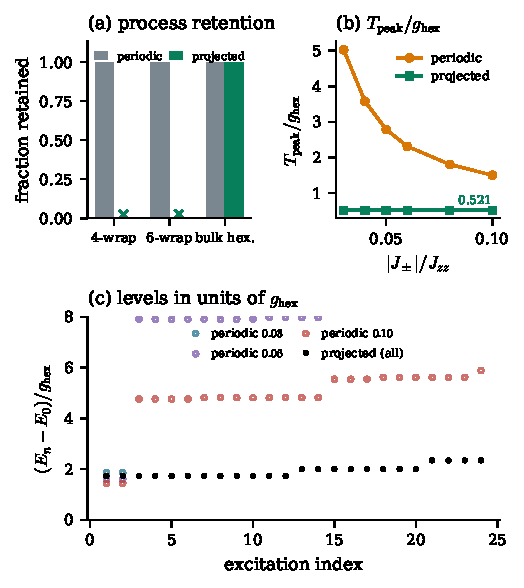
\includegraphics[width=\columnwidth]{fig2_fcc32_benchmark.pdf}
\caption{\textbf{Rigorous FCC-32 benchmark.}
(a) Fraction of each matrix-element channel retained. Gray bars are the
periodic operator; green bars/crosses are the projected operator, which
removes both wrapping channels and leaves the bulk hexagon unchanged.
(b) $T_{\rm peak}/\ghex$ versus $|\Jpm|/\Jzz$. Projection gives the constant
$0.521$ expected for a Hamiltonian proportional to $\ghex$, whereas the
periodic result grows because it also contains $\gfour$. (c) Lowest 24
excitation energies. Open colored points are periodic results at the labeled
$|\Jpm|/\Jzz$; black points are projected results, which coincide for every
coupling when energies are divided by $\ghex$.}
\label{fig:benchmark}
\end{figure}

Figure~\ref{fig:benchmark} asks directly whether the protocol also destroys
physical processes.  Three tests answer no.  First, channel-resolved row
counts show zero retention of the 24 four-loops and 96 wrapping hexagons but
unit retention of all 32 contractible hexagons [Fig.~\ref{fig:benchmark}(a)].
Second, at $\Jpm/\Jzz=-0.05$, explicit $\bdelta=0$ filtering and the parity
mask reduce 91,482 nonzero periodic entries to the same 18,330 entries, with
zero entrywise residual in double precision.  Third, varying
$0.03\leq|\Jpm|/\Jzz\leq0.10$ collapses both the full low-energy spectrum and
the heat-capacity peak onto $\ghex$, giving
$T_{\rm peak}/\ghex=0.52103$ [Figs.~\ref{fig:benchmark}(b,c)].  The periodic
operator cannot collapse because it contains the independent scale
$\gfour$.  Selectivity at the row level and cubic scaling of the resulting
operator provide separate checks that the physical ring dynamics survives.

The same distinction is visible dynamically. To avoid introducing neutron
polarization factors, we compute the longitudinal four-sublattice trace
\begin{align}
 S^{zz}(\bq,\omega)
 &=\frac1N\sum_{n,a}|\mathcal S_{na}(\bq)|^2
 \delta[\omega-(E_n-E_0)],\\
 \mathcal S_{na}(\bq)
 &=\sum_{j\in a}e^{-i\bq\cdot\br_j}\langle n|S_j^z|0\rangle,
\label{eq:dssf}
\end{align}
where $a$ labels the four pyrochlore sublattices. This is a pure pseudospin
correlation: it contains neither local-axis projections nor the laboratory
neutron polarization tensor. The coherent sum $|\sum_a\mathcal S_{na}|^2$
vanishes at the exact FCC-32 momenta by the ice constraint, while the
sublattice trace remains finite.
FCC-32 has only eight independent translation momenta: $\Gamma$, three
symmetry-related $X$ points, and four symmetry-related $L$ points.  We show
only those sectors, not a continuous form-factor interpolation.

\begin{figure}[t]
\centering
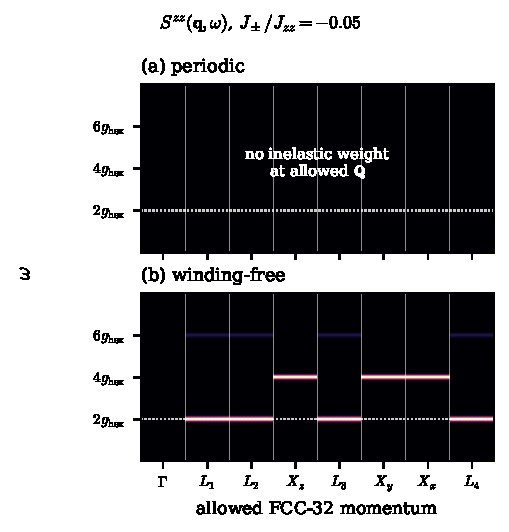
\includegraphics[width=\columnwidth]{fig3_fcc32_dssf.pdf}
\caption{\textbf{FCC-32 spectral response at the eight allowed momenta.}
Periodic and winding-free $S^{zz}(\bq,\omega)$ at
$\Jpm/\Jzz=-0.05$ on common linear scales. The periodic source vanishes at
these momenta; the projected $L$ response begins at the dotted
$\omega=2\ghex$ line and follows the contractible-ring scale.}
\label{fig:dssf}
\end{figure}

Figure~\ref{fig:dssf} shows that cleaning is not a rigid energy rescaling.
The artifact-selected periodic ground state has no inelastic weight in this
$S^{zz}$ trace at the allowed momenta.  Projection restores finite matrix
elements over the contractible-hexagon spectrum, with the first active $L$ line at
$2\ghex$ and cubic symmetry reproduced independently within the three $X$
and four $L$ sectors.  The redistribution of spectral weight, together with
the energy collapse in Fig.~\ref{fig:benchmark}(c), is a dynamical check that
the retained operator is not obtained by simply shifting periodic levels.

We finally apply the scale test to Ce$_2$Hf$_2$O$_7$, whose heat capacity has
maxima near $T_1=0.065$ K and $T_2=0.025$ K \cite{Smith2025}.  The published
seventh-order numerical-linked-cluster (NLC) fit A gives
$(J_a,J_b,J_c)=(0.050,0.021,0.004)$ meV.  Choosing $J_a$ as the dominant gauge
axis gives $\Jzz=J_a$ and $\Jpm=-(J_b+J_c)/4=-0.00625$ meV.  The FCC-32 clean
coefficient then predicts $T_{\rm ring}=7.1$ mK, more than a factor of three
below $T_2$.

The two temperatures therefore constrain different combinations of the same
exchange tensor.  To combine them without pretending to rerun unavailable
NLC internals, we impose three explicit conditions: preserve the leading
high-temperature moment $\sum_\alpha J_\alpha^2$ of set A, preserve its
transverse anisotropy $J_b-J_c$, and set the clean FCC-32 ring maximum to
$T_2$.  The unique nearby solution is
\begin{align}
 (J_a,J_b,J_c)_{A^\star}&=(0.04644,0.02661,0.00961)\ {\rm meV},\\
 J_\pm^\star&=-0.00906\ {\rm meV}.
\end{align}

\begin{figure}[t]
\centering
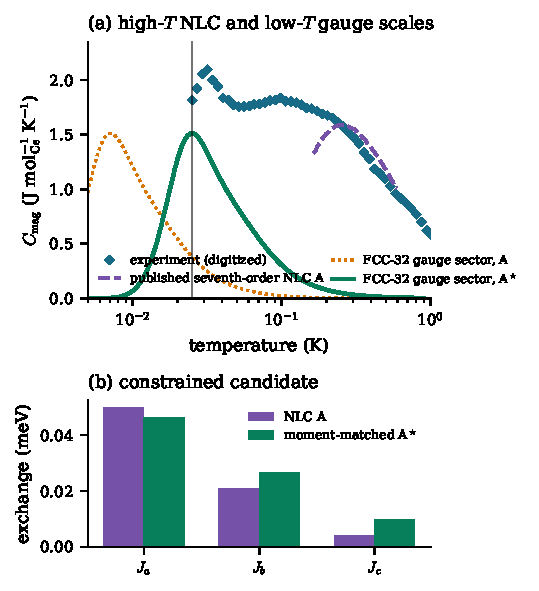
\includegraphics[width=\columnwidth]{fig4_ce2hf2o7.pdf}
\caption{\textbf{Joint constraint for Ce$_2$Hf$_2$O$_7$.}
(a) Heat-capacity points and the published NLC-A curve digitized from
Ref.~\cite{Smith2025} for visual comparison, with the clean FCC-32 gauge
contributions for A and A$^\star$.  The line marks $T_2=25$ mK.
(b) A$^\star=(0.04644,0.02661,0.00961)$ meV preserves
$\sum_\alpha J_\alpha^2$ and $J_b-J_c$ of A while moving the clean ring peak
to $T_2$.  The A$^\star$ bars are a parameter target, not a completed NLC
curve.}
\label{fig:material}
\end{figure}

Figure~\ref{fig:material} separates the established calculation from the
proposed material inference.  The published NLC-A curve describes the
higher-temperature feature, but its clean low-energy ring scale misses the
second peak.  A$^\star$ is a better joint-scale candidate because it retains
the leading high-temperature moment while satisfying the observed
low-temperature constraint.  A new seventh-order NLC evaluation at
A$^\star$ is the decisive test of whether the full high-$T$ line shape is
also retained; no such curve is claimed here.

The central result is therefore methodological and falsifiable.  On FCC-32,
the leading weak-coupling error is a lower-order topological exchange, not a
small shift of the bulk spectrum.  The transported-dipole projector removes
that channel exactly through third order while leaving every physical
hexagon matrix element intact.  Its thermodynamic and spectroscopic
consequences turn the lower Ce$_2$Hf$_2$O$_7$ peak into a quantitative
constraint for a joint NLC and winding-free fit.

\begin{acknowledgments}
[Acknowledgments.]
\end{acknowledgments}

\bibliography{references}

\end{document}
